% Clase y configuracion de tipo de documento
\documentclass[10pt,a4paper,spanish]{article}
% Inclusion de paquetes
\usepackage{a4wide}
\usepackage{amsmath, amscd, amssymb, amsthm, latexsym}
\usepackage[spanish]{babel}
\usepackage[utf8]{inputenc}
\usepackage[width=15.5cm, left=3cm, top=2.5cm, height= 24.5cm]{geometry}
\usepackage{fancyhdr}
\pagestyle{fancyplain}
\usepackage{listings}
\usepackage{enumerate}
\usepackage{xspace}
\usepackage{longtable}
\usepackage{caratula}
\usepackage{hyperref}
\usepackage{graphicx}
\graphicspath{{img/}}
\usepackage{pgfplots}

\usepackage{color} % para snipets de codigo coloreados
\usepackage{fancybox}  % para el sbox de los snipets de codigo

\definecolor{litegrey}{gray}{0.94}

% \newenvironment{sidebar}{%
% 	\begin{Sbox}\begin{minipage}{.85\textwidth}}%
% 	{\end{minipage}\end{Sbox}%
% 		\begin{center}\setlength{\fboxsep}{6pt}%
% 		\shadowbox{\TheSbox}\end{center}}
% \newenvironment{warning}{%
% 	\begin{Sbox}\begin{minipage}{.85\textwidth}\sffamily\lite\small\RaggedRight}%
% 	{\end{minipage}\end{Sbox}%
% 		\begin{center}\setlength{\fboxsep}{6pt}%
% 		\colorbox{litegrey}{\TheSbox}\end{center}}

\newenvironment{codesnippet}{%
	\begin{Sbox}\begin{minipage}{\textwidth}\sffamily\small}%
	{\end{minipage}\end{Sbox}%
		\begin{center}%
		\vspace{-0.4cm}\colorbox{litegrey}{\TheSbox}\end{center}\vspace{0.3cm}}




% Encabezado
\lhead{Organización del Computador II}
\rhead{Grupo: Fuga Villera Nro. 2}
% Pie de pagina
\renewcommand{\footrulewidth}{0.4pt}
\lfoot{Facultad de Ciencias Exactas y Naturales}
\rfoot{Universidad de Buenos Aires}

\begin{document}

% Datos de caratula
\materia{Organización del Computador II}
\titulo{Trabajo Práctico 2: Experimentos}
%\subtitulo{}
\grupo{
	Grupo: Fuga Villera Nro. 2
	\href{https://www.youtube.com/watch?v=wBNjDRXJNyY}{
		
\includegraphics[height=0.4cm,keepaspectratio]{YouTube-icon-full_color.png}
	}
}

\integrante{Gabriel Matles}{397/12}{gabriel29m@gmail.com}
\integrante{Manuel Mena}{313/14}{manuelmena1993@gmail.com}
\integrante{Francisco Demartino}{348/14}{demartino.francisco@gmail.com}

\maketitle

\newpage

% Para crear un indice
\tableofcontents

% Forzar salto de pagina
\clearpage

\section{Objetivos generales}

El objetivo de este trabajo práctico es evaluar la eficiencia del modelo de programación SIMD mediante la implementación de diversos algoritmos en lenguaje Ensamblador utilizando instrucciones SSE. \\
\indent Las mediciones se realizan mediante pruebas empíricas del código frente a algoritmos que cumplen la misma especificación, implementados en un lenguaje de alto nivel (C). \\
\indent En este proyecto, los algoritmos a implementar se basaron en el procesamiento de imágenes, en el cual el uso del modelo SIMD es provechoso.

\section{Calidad de las Mediciones}
Antes de medir tiempos y sacar conclusiones de los mismos, es importante tener un esquema básico de como se realizarán las mediciones en el presente trabajo, y bajo que condiciones. \\

\textbf{Características de la computadora en la que los experimentos fueron realizados:} \\
\textit{Procesador:} Intel Core i7 x8 CPUs 2GHz \\
\textit{Memoria RAM:} 8 GB \\
\textit{Sistema operativo:} Ubuntu 14.04 64 bits. \\

Las mediciones se realizaron corriendo los filtros 1000 veces para el \textit{Diff} y 100 para el \textit{Blur}. Se realizó un promedio, y estos promedios son los que se pueden apreciar en los distintos gráficos. Los tiempos están medidos en ciclos de clock.

\section{Experimentación}

Los experimentos realizados se dividen dos ramas: en comparar los filtros implementados en C contra los implementados en ASM, y comparar específicamente sobre filtro blur, las distintas implementaciones del mismo. \\

En cuanto a las implementaciones del blur, lo que hicimos fue alternar la forma en la que recorrimos la matriz de convolucion para calcular el valor de cada pixel. En la primer implementación la recorrimos desplazandonos por cada fila hasta llegar al borde derecho y pasar a la suguiente fila. En la otra, en cambio, nos desplazamos por columna (DE ESTO QUIZAS PODRIA HACERSE UN GRAFICO QUE LO ILUSTRE MEJOR, SOBRE TODO LA PARTE DE QUE AGARRAMOS DE A 4 DE UNA MISMA FILA PERO EL MOVIMIENTO ES DE COLUMNA) hasta llegar a la ultima fila y ahi seguimos con las siguientes 4 columnas. \\

Es necesario destacar dos cosas: gracias a las operaciones SSE podemos computar 4 pixeles simultaneamente, pero estos pixeles son contiguos en memoria, lo que equivale a que estan uno al lado del otro horizontalmente en la imagen. Es por esto que una vez que termino de recorrer la columna, la siguiente será la que se encuentra a 4 posiciones de distancia.
¿HIPOTESIS?:La forma en la que se almacena y se vacía la memoria caché se ve afecatada por la forma en que recorramos la matriz, ya que al hacer un recorrido contiguo en memoria, equivalente a recorrer la imagen horizontalmente, tendrá un mayor hitrate que si la recorremos verticalmente, ya que al no ser contiguas se deberán leer de memoria varios bloques que puedan no encontrarse almacenados. Esto representaría una baja en la performance temporal del algoritmo. \\

C vs ASM

\begin{enumerate}
	\item Medir los tiempos que tardan los distintos filtros para distintos tamaños de imágenes y para imágenes diferentes. Este experimento tiene como objetivo tener una idea del tiempo de ejecución del algoritmo en general, y comparandolo con otras implementaciones del mismo, tener una idea de cual tiene mejor tiempo de ejecución.
	\item Medir y comparar la memoria utilizada por cada filtro
	\item Registrar la precisión que pueda perderse en cada lenguaje
	\item Repetir los experimentos utilizando la optimización O3 para C
\end{enumerate}

ASM vs ASM

\begin{enumerate}
	\item Medir los tiempos que tardan ambas implementaciones del filtro blur
	\item Registrar el comportamiento de la memoria caché frente a las distintas formas de recorrer las matrices para las implementaciones del filtro blur
\end{enumerate}

\section{Diff}

\subsection{Introducción}

\textit{Diff} es un filtro que genera una imagen que, por medio de una escala de grises, indica dónde difieren las imágenes y qué tanto.
La intensidad del gris está dada por la maxima diferencia entre las componentes de los pixeles de ambas imágenes. \\

Esta es la imagen que genera el filtro al pasarle las imágenes lena24.bmp y colores24.bmp \\

\begin{center}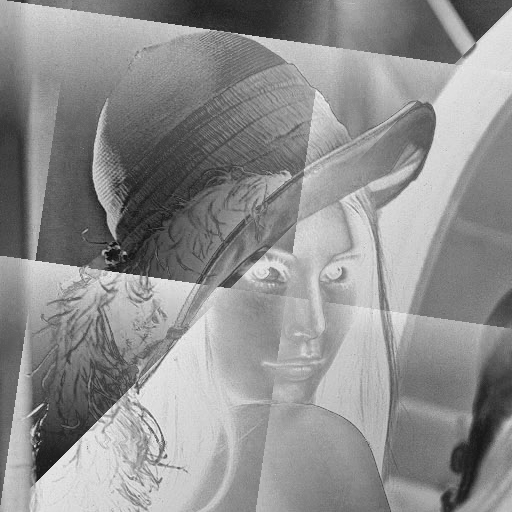
\includegraphics[keepaspectratio]{diff_lena24_colores24.png}\end{center}

\subsection{Implementación en C}

Se tienen dos indices (x e y) para recorrer las imágenes. Dentro del ciclo, para cada para de pixeles se calculan las diferencias entre las componentes y se toma la maxima. Luego se almacena 255 en alpha y el valor calculado en las otras 3 componentes en la imagen de salida. \\

Este es el pseudocódigo para cada iteración del ciclo:

\begin{codesnippet}
\begin{verbatim}

maximo = max(max(abs(src_matrix[y][x+B] - src_2_matrix[y][x+B]),
                 abs(src_matrix[y][x+G] - src_2_matrix[y][x+G])),
                 abs(src_matrix[y][x+R] - src_2_matrix[y][x+R]));

dst_matrix[y][x+B] = maximo;
dst_matrix[y][x+G] = maximo;
dst_matrix[y][x+R] = maximo;
dst_matrix[y][x+A] = 255;

\end{verbatim}
\end{codesnippet}

\subsection{Implementación en ASM}

La implementación en ASM consiste en aprovechar las instrucciones SSE para poder leer de a 4 pixeles. Como debemos restar las componentes, es necesario desempaquetar esos 4 pixeles, es decir pasarlos a 2 registros donde podamos manejar cada componente como word, no como byte. Ya que de otra forma podríamos estar perdiendo información. Esto hace que por mas que podamos leer de a 4, solo podamos computar de a 2 en simultáneo.

\begin{codesnippet}
\begin{verbatim}

; Traigo 4 pixeles de cada imagen desde la memoria
movups xmm1, [rdi]     ; rdi = puntero a imagen 1
movups xmm2, [rsi]     ; rsi = puntero a imagen 2

; Desempaqueto los pixeles para poder hacer la resta sin perder informacion
movups xmm3, xmm1
movups xmm4, xmm2

punpcklbw xmm1, xmm5   ; xmm5 esta limpio para
punpckhbw xmm3, xmm5

punpcklbw xmm2, xmm5
punpckhbw xmm4, xmm5

\end{verbatim}
\end{codesnippet}

Luego procede a hacer la resta entre las componentes, obtener su valor absoluto y empaquetarlo en un único registro

\begin{codesnippet}
\begin{verbatim}

; Resto los pixeles de ambas imágenes. El resultado queda en xmm1 y xmm3
psubw xmm1, xmm2
psubw xmm3, xmm4

; Obtengo el valor absoluto de la resta de los pixeles
pabsw xmm1, xmm1
pabsw xmm3, xmm3

; Empaqueto el resultado nuevamente en un solo registro.
packuswb xmm1, xmm3

\end{verbatim}
\end{codesnippet}

Para buscar la máxima diferencia es necesario hacer una copia del registro, comparar un canal con el otro, y el resultado compararlo con el canal restante

\begin{codesnippet}
\begin{verbatim}

; Copio xmm1 en xmm2 para poder buscar el maximo
movups xmm2, xmm1

; Comparo el canal R con el canal G y luego el resultado lo comparo con el canal B
psrldq xmm2, 1		; Me muevo un byte a la derecha
pmaxub xmm1, xmm2
psrldq xmm2, 1		; Me muevo un byte a la derecha
pmaxub xmm1, xmm2

; Pongo el maximo que hasta ahora tengo en el canal R de cada pixel en todos los canales
pshufb xmm1, xmm7   ; xmm es la mascara que distribuye el valor del maximo en
                    ; todas las componentes

\end{verbatim}
\end{codesnippet}

Finalmente se inserta el alpha con valor 255 y se guarda

\begin{codesnippet}
\begin{verbatim}

pinsrb xmm1, eax, 3     ; eax = 255
pinsrb xmm1, eax, 7
pinsrb xmm1, eax, 11
pinsrb xmm1, eax, 15

; Muevo los pixeles con el filtro aplicado a dst
movups [r9], xmm1       ; r9 = puntero a imagen destino

\end{verbatim}
\end{codesnippet}

\section{Blur}

\subsection{Introducción}

\textit{Blur} es un filtro que suaviza una imagen. Consta de asignarle a cada componente de la imagen de salida el promedio de la vecindad del mismo en la imagen original. En este trabajo práctico tomaremos el promedio ponderado, para lograr un desenfoque más natural. Se lo llama \textit{Blur Gaussiano} ya que la matriz que se utiliza para calcular este promedio es calculada a partir de una función Gaussiana. \\

Los bordes de la imagen no se veran afectados por el filtro ya que en esas posiciones de la imagen no se puede tomar la cantidad de vecinos necesaria. \\

El filtro toma además de la imagen otros 2 parámetros de entrada: $ \sigma $ y radio. \\

El parámetro $ \sigma $ determina cuánto se suaviza la imagen, ya que es el valor que modifica, a través de la función Gaussiana, el contenido de la matriz utilizada para la convolución. Dado que dicha función integra a 1, decimos que esta convolución es un promedio ponderado; esto garantiza que el brillo de la imagen no se altera.\\

El radio representa la distancia desde el pixel hasta su último vecino. En otras palabras, determina el tamaño de los lados de la matriz (es una matriz cuadrada): 2 * radio + 1. \\

Esta es la imagen que genera el filtro para la imagen lena24.bmp con parametro $ \sigma $ = 5 y r = 15 \\

\begin{center}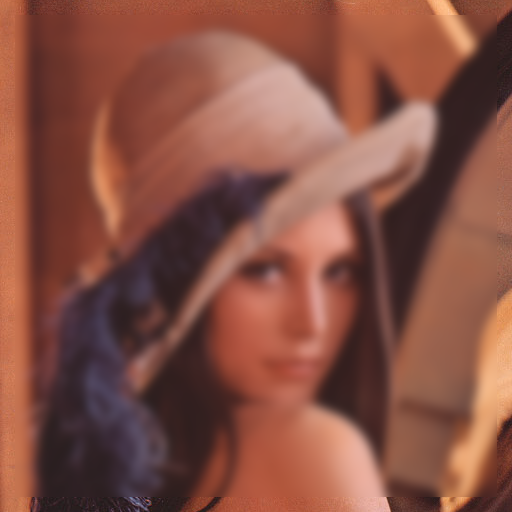
\includegraphics[keepaspectratio]{blur_lena24_5_15.png}\end{center}

\subsection{Implementación en C}

En la implementación en C, el cálculo de cada pixel consiste en recorrer los pixeles vecinos utilizando dos índices (x e y), acumular el valor del producto entre cada una de las componentes del pixel y el valor correspondiente de la matriz de convolución, y una vez terminado el recorrido, escribir en la imagen de salida el resultado acumulado para cada una de las componentes. \\

Este es el pseudocódigo de cada iteración del ciclo:

\begin{codesnippet}
\begin{verbatim}

blue = 0
green = 0
red = 0

for x from -radius to radius inclusive do:
  for y from -radius to radius inclusive do:

      blue  += (src_matrix[row + y][(col + x) * 4 + OFFSET_BLUE]) *
                conv_matrix[radius - y][radius - x];

      green += (src_matrix[row + y][(col + x) * 4 + OFFSET_GREEN]) *
                conv_matrix[radius - y][radius - x];

      red   += (src_matrix[row + y][(col + x) * 4 + OFFSET_RED]) *
                conv_matrix[radius - y][radius - x];

dst_matrix[row][col * 4 + OFFSET_BLUE]  = blue;
dst_matrix[row][col * 4 + OFFSET_GREEN] = green;
dst_matrix[row][col * 4 + OFFSET_RED]   = red;
dst_matrix[row][col * 4 + OFFSET_ALPHA] = 255;

\end{verbatim}
\end{codesnippet}

\subsection{Implementación 1 en ASM}

La primera implementación en ASM consiste en procesar el pixel recorriendo la matriz de convolucion fila por fila, cada una de izquierda a derecha.
Calcula un pixel de la imagen de salida a la vez. La ventaja que sacamos de las instrucciones SSE es que para procesar cada fila podemos computar 4 pixeles de la imagen de entrada simultáneamente. \\

Esta implementación consumió mucho tiempo de trabajo. Mas adelante analizaremos si los resultados justifican la dificultad de desarrollar y pensar usando el model SIMD. \\

Cada pixel tiene 4 componentes, cada una ocupa un byte, por lo que cada pixel ocupa 4 bytes. Dentro de los registros xmm podemos almacenar hasta 16 bytes, por lo que es posible guardar dentro el valor de 4 pixeles. De esta forma podemos obtener el valor de 4 pixeles que serán procesados acorde al uso del modelo SIMD. \\

Para calcular el valor final de cada pixel, nuestra implementación usa 2 indices que representaran la posición actual (x,y) y que utilizamos para recorrer los vecinos. Dentro de el ciclo del recorrido, lee de memoria 4 pixeles y los almacena en un registro xmm para luego copiarlo en otros 3 que usaremos para separarlos por componente (no son 4 ya que la componente alpha tiene como valor 255 siempre).

\begin{codesnippet}
\begin{verbatim}

movdqu xmm3, [r12+r10*PIXEL_SIZE]   ; xmm3 = vector imagen entrada
                                    ; r12  = puntero de la imagen de entrada
                                    ; r10  = posicion en la imagen d entrada

movdqu xmm5, xmm3                   ; xmm5 va a contener solo las componentes azules
movdqu xmm6, xmm3                   ; xmm6 va a contener solo las componentes verdes
movdqu xmm7, xmm3                   ; xmm7 va a contener solo las componentes rojas

; xmm13, xmm14 y xmm15 contienen mascaras para hacer el shuffle
pshufb xmm5, xmm13                  ; xmm5 = B0 0 0 0 B1 0 0 0 B2 0 0 0 B3 0 0 0
pshufb xmm6, xmm14                  ; xmm6 = G0 0 0 0 G1 0 0 0 G2 0 0 0 G3 0 0 0
pshufb xmm7, xmm15                  ; xmm7 = R0 0 0 0 R1 0 0 0 R2 0 0 0 R3 0 0 0

; Convierto a float
cvtdq2ps xmm5, xmm5
cvtdq2ps xmm6, xmm6
cvtdq2ps xmm7, xmm7

\end{verbatim}
\end{codesnippet}

En este punto tenemos separadas las componentes de los 4 pixeles en 3 registros distintos (uno por componente). Resta multiplicarlas por las posiciones correspondientes de la matriz de convolucion y acumularlas. \\

Para ello usamos la instruccion dpps. Esta instrucción toma 3 parametros: el registro destino, el registro fuente y un inmediato de un byte. Hace el prouducto interno entre ambos registros, y según el inmediato se define cuales de las 4 posiciones se emplean para hacer la cuenta y en cuál se almacena. El nibble más significativo indica qué cuentas se hacen, por ejemplo F se toman todas y 5 sólo la primera y tercera. El nibble menos significativo indica la posición en la que se almacena. \\

Lo conveniente de esta instruccion es que nos permite hacer las sumas de los productos simultáneamente y almacenarla donde queramos dentro del registro. Esto es muy bueno ya que podemos almacenarla en posiciones distintas dependiendo de que componente estemos computando, para despues sumar los 3 registros en uno y que nos quede el pixel.

También es muy útil para poder manipular la lecura de los ultimos valores de la matriz. Ya que leemos de a 4, pero en el ultimo caso de cada fila podemos estar queriendo computar 3 o 1 pixel. Esta instrucción nos lo facilita ya que podemos indicar cuales tener en cuenta para el producto interno y cuales no. \\

\begin{codesnippet}
\begin{verbatim}

; Voy multiplicando 4 vs 4 entre convolucion y componente k de cada pixel
dpps xmm5, xmm4, 0xF1               ; en xmm4 tengo los 4 valores correspondientes
dpps xmm6, xmm4, 0xF2               ; de la matriz de convolucion
dpps xmm7, xmm4, 0xF4

addps xmm0, xmm5                    ; xmm0 contendra mi pixel final
addps xmm0, xmm6
addps xmm0, xmm7

\end{verbatim}
\end{codesnippet}

Una vez calculado el pixel, convierte los valores del registro xmm0 en formato int de 4bytes, lo empaqueta y le agrega el valor de alpha, que es 255. Finalmente lo guarda en la matriz de salida

\section{Problemas}

Se nos presentaron varios problemas durante el desarrollo del filtro \textit{Blur} en lenguaje ensamblador. \\

Comenzamos teniendo un problema a la hora de almacenar los valores, lo que nos resultaba en una imagen con una gran cantidad de pixeles apagados. \\

\begin{center}
\includegraphics[width=7cm, keepaspectratio]{problema_colores.jpg} \\\end{center}

Conseguimos solucionarlo pero aún el filtro no era capaz de manipular correctamente los vectores que se leían de los píxeles vecinos. Las máscaras que utilizabamos para hacer el shuffle no eran correctas, y nos daba esta salida como resultado: \\

\begin{center}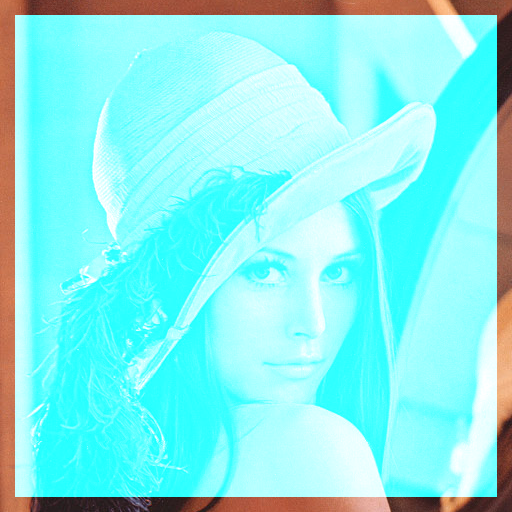
\includegraphics[width=10cm, keepaspectratio]{problema_lena_cristal.png} \\\end{center}

Resolvimos el problema de las máscaras, pero aun así el filtro no desenfocaba la imagen, sino que le daba otro tipo de efecto. \\

\begin{center}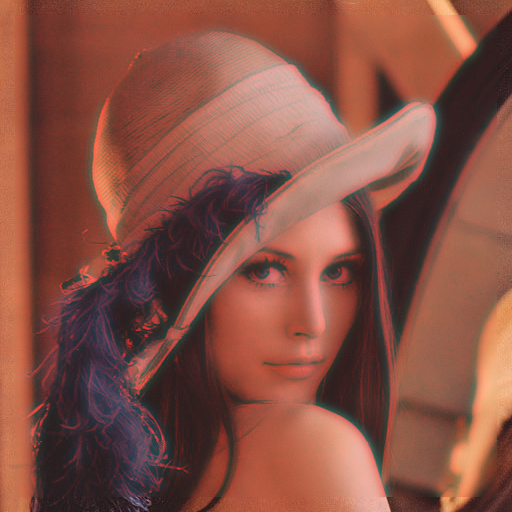
\includegraphics[width=10cm, keepaspectratio]{problema_lena.png} \\\end{center}

El programa no recorría correctamente los vecinos, no entendíamos porqué, asi que lo rehicimos y obtuvimos esta salida: \\

\begin{center}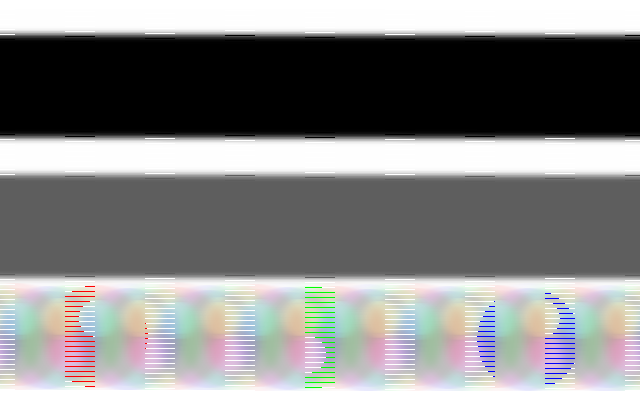
\includegraphics[width=15cm, keepaspectratio]{problema_circulos_columnas.png} \\\end{center}

Este fue el último percance que tuvimos que enfrentar. Estabamos recorriendo de a 16 pixeles en lugar de a 4. El tiempo empleado en solucionar estos errores nos dió a conocer la dificultad de trabajar con vectores utilizando SIMD, y la forma en que se multiplica la cantidad de factores que tenemos que tener en cuenta para realizar una tarea que, por ejemplo, en C resulta muy sencilla y fácil de entender. \\

Si comparamos el modo en que desarrollamos en cada lenguaje, en lenguaje ensamblador sufrimos muchos errores, aún implementando paso por paso y con cautela, cuando en C los filtros quedaron terminados en cuestion de minutos.

\section{Resultados}

Se realizaron una serie de experimentos para poder conocer qué ventajas presenta el uso del modelo SIMD. Para ello comparamos sobre ambos filtros las implementaciones hechas en lenguaje ensamblador, que aprovechan las instrucciones SSE, y las hechas en C, que no tienen esta ventaja. \\

Las hipótesis para ambos filtros no varían.

\subsection{Mediciones}

Realizar una medición de performance \emph{rigurosa} es más difícil de lo que parece. En este experimento deberá realizar distintas mediciones de performance para verificar que sean buenas mediciones. \\

En un sistema ``ideal'' el proceso medido corre solo, sin ninguna interferencia de agentes externos. Sin embargo, una PC no es un sistema ideal. Nuestro proceso corre junto con decenas de otros, tanto de usuarios como del sistema operativo que compiten por el uso de la CPU. Esto implica que al realizar mediciones aparezcan ``ruidos'' o ``interferencias'' que distorsionen los resultados. \\

El primer paso para tener una idea de si la medición es buena o no, es tomar varias muestras. Es decir, repetir la misma medición varias veces. Luego de eso, es conveniente descartar los outliers, que son los valores que más se alejan del promedio. Con los valores de las mediciones resultantes se puede calcular el promedio y también la varianza, que es algo similar el promedio de las distancias al promedio. \\

\subsection{Diferencias de performance en Diff}

Hipótesis: La velocidad de la ejecución del filtro implementado en lenguaje ensamblador será aproximadamente 4 veces la velocidad de la del filtro implementado en C, debido a la capacidad de procesar de a 4 pixeles de manera simultánea que nos proveen las instrucciones SSE. \\

Se corrieron ambas implementaciones 1000 veces utilizando 4 pares de imágenes de distintosº tamaños: 120 x 120, 512 x 512, 640 x 400 y 800 x 600. \\

Las diferencias de performance temporal de las implementaciones en cuanto al filtro \textit{Diff} fueron destacables. La hipótesis fue incorrecta. El filtro implementado en lenguaje ensamblador llegó a superar al implementado en C por más de 10 veces en velocidad. Esto puede apreciarse en el siguiente gráfico. \\
\begin{center}
\begin{tikzpicture}
  \begin{axis}[title  ={ Figura 1 - Cantidad de clocks (toda la imagen), filtro Diff},
    xbar,
    y axis line style = { opacity = 0 },
    axis x line       = none,
    tickwidth         = 0pt,
    enlarge y limits  = 0.2,
    enlarge x limits  = 0.02,
    symbolic y coords = {800 x 600, 640 x 400, 512 x 512, 120 x 120},
    nodes near coords,
  ]
  \addplot coordinates {
    (629234,120 x 120)
    (11413881,512 x 512)
    (11382588,640 x 400)
    (21231368,800 x 600)
  };
  \addplot coordinates {
    (70563,120 x 120)
    (1003030,512 x 512)
    (992484,640 x 400)
    (1945705,800 x 600)
  };
  \legend{C, ASM}
  \end{axis}
\end{tikzpicture}
\end{center}


\begin{center}
\begin{tikzpicture}
  \begin{axis}[title  ={ Figura 2 - Cantidad de clocks (por pixel), filtro Diff},
    xbar,
    y axis line style = { opacity = 0 },
    axis x line       = none,
    tickwidth         = 0pt,
    enlarge y limits  = 0.2,
    enlarge x limits  = 0.02,
    symbolic y coords = {800 x 600, 640 x 400, 512 x 512, 120 x 120},
    nodes near coords,
  ]
  \addplot coordinates {
    (44,120 x 120)
    (43,512 x 512)
    (44,640 x 400)
    (44,800 x 600)
  };
  \addplot coordinates {
    (5,120 x 120)
    (4,512 x 512)
    (4,640 x 400)
    (4,800 x 600)
  };
  \legend{C, ASM}
  \end{axis}
\end{tikzpicture}
\end{center}

\subsection{Diferencias de precisión en Diff}

Se compararon pixel a pixel las imágenes de salida generadas por ambas implementaciones del filtro y no hubo diferencias.

\subsection{Diferencias de performance en Blur}

Hipótesis: La velocidad de la ejecución del filtro implementado en lenguaje ensamblador será aproximadamente 4 veces la velocidad de la del filtro implementado en C, debido a la capacidad de procesar de a 4 pixeles de manera simultánea que nos proveen las instrucciones SSE. \\

Se corrieron ambas implementaciones 100 veces utilizando 4 pares de imágenes de distintosº tamaños: 120 x 120, 512 x 512, 640 x 400 y 800 x 600. Decidimos bajar el numero de repeticiones con respecto al filtro \textit{Diff} ya que este filtro demora más en generar un resultado.\\

Las diferencias de performance temporal de las implementaciones en cuanto al filtro \textit{Blur} fueron importantes, aunque no tanto como lo fueron para el filtro \textit{Diff}. La hipótesis, una vez más, fue incorrecta. El filtro implementado en lenguaje ensamblador nuevamente superó con gran amplitud al implementado en C, ejecutándose alrededor de 9 veces mas rápido. \\
\begin{center}
\begin{tikzpicture}
  \begin{axis}[title  ={ Figura 3 - Cantidad de clocks (toda la imagen), filtro Blur},
    xbar,
    y axis line style = { opacity = 0 },
    axis x line       = none,
    tickwidth         = 0pt,
    enlarge y limits  = 0.2,
    enlarge x limits  = 0.02,
    symbolic y coords = {800 x 600, 640 x 400, 512 x 512, 120 x 120},
    nodes near coords,
  ]
  \addplot coordinates {
    (228968528,120 x 120)
    (6652537344,512 x 512)
    (7039704576,640 x 400)
    (13256412160,800 x 600)
  };
  \addplot coordinates {
    (27778298,120 x 120)
    (812709312,512 x 512)
    (815566272,640 x 400)
    (1499686144,800 x 600)
  };
  \legend{C, ASM}
  \end{axis}
\end{tikzpicture}
\end{center}

\begin{center}
\begin{tikzpicture}
  \begin{axis}[title  ={ Figura 4 - Cantidad de clocks (por pixel), filtro Blur},
    xbar,
    y axis line style = { opacity = 0 },
    axis x line       = none,
    tickwidth         = 0pt,
    enlarge y limits  = 0.2,
    enlarge x limits  = 0.02,
    symbolic y coords = {800 x 600, 640 x 400, 512 x 512, 120 x 120},
    nodes near coords,
  ]
  \addplot coordinates {
    (15900,120 x 120)
    (25377,512 x 512)
    (27498,640 x 400)
    (27617,800 x 600)
  };
  \addplot coordinates {
    (1929,120 x 120)
    (3100,512 x 512)
    (3185,640 x 400)
    (3124,800 x 600)
  };
  \legend{C, ASM}
  \end{axis}
\end{tikzpicture}
\end{center}

\subsection{Diferencias de precision en Blur}

Una vez más comparamos las imágenes de salida generadas por ambas implementaciones y esta vez sí obtuvimos diferencias. Si bien eran casi imperceptibles para el ojo humano, en cada imagen encontramos muchos pares de pixeles que diferían entre sí por un valor de 1 en alguna componente del color.




\subsection{Optimización O3 para la implementación en C}

En el momento de compilar el programa, existe un parametro que controla el nivel de optimización en el código. Al cambiar este valor, la compilación de código tomará algo más de tiempo, y utilizará mucha más memoria, especialmente al incrementar el nivel de optimización. Hablamos de la variable -O. Existen siete ajustes para -O: -O0, -O1, -O2, -O3, -Os, -Og y -Ofast. \\

Con motivo de comparar que tanto es posible optimizar el código, y si en verdad lleva a una mejoría en la performance, compilamos los filtros con la optimización -O3 y registramos su el tiempo en ciclos de clock que toma cada uno. \\

-O3 es el nivel más alto de optimización posible. Activa opitimizaciones que son caras en términos de tiempo de compilación y uso de memoria. Aún así, no garantiza una forma de mejorar el rendimiento y, de hecho, en muchos casos puede ralentizar un sistema debido al uso de binarios de gran tamaño y mucho uso de la memoria. También se sabe que -O3 puede romper algunos paquetes por lo que no es recomendado su uso, pero justamente para conocer cuánto valen estos riesgos es que llevamos adelante este experimento. \\

Los resultados que obtuvimos fueron los esperados. Este nivel de optimización reflejó una mejora en la velocidad del algoritmo, pero no la suficiente como para vencer a la implementación en lenguaje ensamblador. \\

En la figura 6 podemos ver que, al considerar el tiempo por pixel, la imagen más chica se procesa más rapido. Esto probablemente se deba a que entra mejor en la caché del microprocesador al ser mas pequeña. \\

Elegimos el filtro \textit{Blur} para este experimento porque es el que mayor tiempo necesita para completarse, siendo así un mejor candidato para resaltar las diferencias de performance temporal. \\
\begin{center}
\begin{tikzpicture}
  \begin{axis}[title  ={ Figura 5 - Cantidad de clocks (toda la imagen), filtro Blur},
    xbar,
    y axis line style = { opacity = 0 },
    axis x line       = none,
    tickwidth         = 0pt,
    enlarge y limits  = 0.2,
    enlarge x limits  = 0.02,
    symbolic y coords = {800 x 600, 640 x 400, 512 x 512, 120 x 120},
    nodes near coords,
  ]
  \addplot coordinates {
    (228968528,120 x 120)
    (6652537344,512 x 512)
    (7039704576,640 x 400)
    (13256412160,800 x 600)
  };
  \addplot coordinates {
    (184060624,120 x 120)
    (5291840000,512 x 512)
    (5328648192,640 x 400)
    (10184464384,800 x 600)
  };
  \addplot coordinates {
    (27778298,120 x 120)
    (812709312,512 x 512)
    (815566272,640 x 400)
    (1499686144,800 x 600)
  };
  \legend{C, C -O3, ASM}
  \end{axis}
\end{tikzpicture}
\end{center}

\begin{center}
\begin{tikzpicture}
  \begin{axis}[title  ={ Figura 6 - Cantidad de clocks (por pixel), filtro Blur},
    xbar,
    y axis line style = { opacity = 0 },
    axis x line       = none,
    tickwidth         = 0pt,
    enlarge y limits  = 0.2,
    enlarge x limits  = 0.02,
    symbolic y coords = {800 x 600, 640 x 400, 512 x 512, 120 x 120},
    nodes near coords,
  ]
  \addplot coordinates {
    (15901,120 x 120)
    (25377,512 x 512)
    (27499,640 x 400)
    (27618,800 x 600)
  };
  \addplot coordinates {
    (12782,120 x 120)
    (20187,512 x 512)
    (20815,640 x 400)
    (21218,800 x 600)
  };
  \addplot coordinates {
    (1929,120 x 120)
    (3100,512 x 512)
    (3186,640 x 400)
    (3124,800 x 600)
  };
  \legend{C, C -O3, ASM}
  \end{axis}
\end{tikzpicture}
\end{center}

\section{Conclusión}

Los resultados de nuestras mediciones han demostrado que la implementación de los filtros en Lenguaje Assembler han logrado una performance de alto nivel de rendimiento ya que el tiempo necesario para su ejecución fue alrededor de 10 veces menor. Si bien, hubo casos donde usando un flag de optimización adecuado al momento de compilar se lograron resultados con un tiempo de ejecución menor, no fue lo suficiente como para superar la velocidad conseguida por el modelo SIMD. \\

Dada la popularidad de la arquitectura de 64 bits de intel, se puede concluir que la implementación del SIMD en assembler tiene un precio razonable frente a la perfomance alcanzada.\\

A pesar de la mayor dificultad para implementar y pensar cómo trabajar con vectores utilizando SIMD, la diferencia de performance es muy notoria, por lo que vale la pena para este tipo de aplicaciones, donde se realiza numerosas veces la misma aritmética.

% \section{Observaciones}
% 	\begin{center}\includegraphics[keepaspectratio]{gen/diff.png}\end{center}
% 	\begin{enumerate}
% 		\item un item
% 		\item otro item
% 	\end{enumerate}

% \section{Resolución}

% \vspace*{0.3cm}
% $xmm0=  0|b_{sup1}$ $g_{sup1}$ $r_{sup1}$ $a_{sup1}$

% % \subsection{Ejercicio X}

% \subsection{Auxiliares}

\end{document}
